%\section{Theoretical Introduction}
\label{sec:cap3}

This chapter presents the theoretical background necessary to understand the techniques and concepts explored in this dissertation. Introduces the reliability challenges of \gls{cots} \gls{sram} \glspl{fpga}, examines fault-tolerance techniques such as N-Modular Redundancy (NMR) and Dynamic Partial Reconfiguration (DPR), discusses memory scrubbing mechanisms, and outlines the principles of fault injection for resilience evaluation.

\section{\glsentrytext{fpga}}
This section introduces the \gls{fpga} architecture, focusing on the role of configurable logic blocks, routing resources, and configuration memory.

A \gls{fpga} is a reconfigurable logic device or a programmable \gls{ic} widely used for the implementation of digital systems.

\glspl{fpga} could be reconfigured by the user, even after deployment \cite{Mazzeo2019}. Its programmable nature enables rapid prototyping, hardware acceleration, and long-term design flexibility.

\glspl{fpga} are successful platforms because they combine the flexibility of software with the speed of hardware, providing adaptable computing cores and high-throughput processing of data streams. They are particularly attractive compared to \glspl{asic} due to their shorter development time and costs, and their ability to be reconfigured \cite{8524728}.

The main advantage of \glspl{fpga} over software-based implementations lies in their inherently parallel architecture, which allows computations to be executed concurrently. For applications that can exploit this parallelism, \glspl{fpga} offer significant performance advantages.

\subsection{Core Structure and Components}

An \gls{fpga} is essentially a complex heterogeneous device implemented on a single chip. Its basic structure consists of an array or matrix of configurable interconnected elements, as illustrated in Figure~\ref{fpga-arch}.

\subsubsection{Configurable Logic Blocks}
These are the elementary logic blocks used to implement the desired logic functions. The \glspl{clb} (sometimes called Logic Cells or Logic Array Blocks, depending on the \gls{fpga}'s manufacturer) perform simple combinational and sequential logic.

In the Zynq 7000 \gls{soc}, \gls{clb} contains a pair of slices, and each of the slices contains four 6-inputs \glspl{lut} and eight storage elements \cite{AMD_UG585}.

These two slices do not have connections between them and are organized by columns, as illustrated in Figure~\ref{fpga-arch-clb-slice-amd}, and have the following features:

\begin{itemize}
    \item Can be configured as a single 6-input \gls{lut} or two 5-input \glspl{lut};
    \item storage elements (memory capability);
    \item Register (\gls{ff}) and shift register available.
\end{itemize}

A \gls{lut} with $m$ inputs can implement any Boolean function defined over those $m$ variables. For example, a 6-input \gls{lut} can realize any six-variable Boolean function, two arbitrary five-variable functions if they share common inputs, or two independent Boolean functions of up to three and two inputs, respectively \cite{Battezzati2010, Mazzeo2019, AMD_UG585}.

The \glspl{lut} could also be configured for other structures, including the so called distributed memory, where each SLICE could be configured as a 64-bit \gls{ram} and as a 32-bit shift register (SRL32) or two 16-bit (SRL16).

\begin{figure}[ht]
\centering
\includegraphics[width=0.75\textwidth]{Cap3/Arrangement-of-Slices-within-the-CLB.png}
\caption{Structure of a \gls{clb} in an AMD's 7-series \gls{fpga}. Reproduced from \textcite{AMD_UG474}.}\label{fpga-arch-clb-slice-amd}
\end{figure}

\subsubsection{Routing and Interconnect Resources}
These resources, including \glspl{sb}, \glspl{cb}, and \glspl{pip}, form a network that electrically interconnects the \glspl{clb}, I/O blocks, and embedded resources to implement complex systems.

\subsubsection{Input/Output Blocks (IOBs)}
These blocks are positioned around the logic core to interface the internal logic with the external environment, handling data input and output.

\subsubsection{Specialized Heterogeneous Resources}
Modern \glspl{fpga} also include various specialized resources beyond the basic structure, such as:
\begin{itemize}
    \item \textbf{Embedded Memories}, such as \glspl{bram}.
    \item \textbf{Arithmetic Resources}, such as \gls{dsp} units.
    \item \textbf{Processing Resources}, which can be hard cores (e.g., ARM Cortex processors in Xilinx Zynq-7000 \gls{apsoc}) or soft processors implemented using programmable logic.
    \item \textbf{Clock-management resources}.
\end{itemize}

As illustrated in Figure~\ref{fpga-arch}, the \gls{fpga} architecture consists of configurable logic blocks, routing resources, and \gls{io} blocks.

\begin{figure}[ht]
\centering
\includegraphics[width=0.75\textwidth]{Cap3/fpga-structure.png}
\caption{\gls{fpga} Structure. Adapted from \textcite{Marioli2010}.}\label{fpga-arch}
\end{figure}

As illustrated  in Figure~\ref{fpga-column-asmbl}, the \gls{fpga} architecture has other specialized hardware, AMD's 7-series is totally based on the columnar approach provided by the \gls{asmbl} architecture. The different domains, represents the diverse platforms with varying feature mixes optimized for different application domains \cite{AMD_UG474}.

\begin{figure}[ht]
\centering
\includegraphics[width=1\textwidth]{Cap3/X30271-ASMBL-Architecture.png}
\caption{\gls{fpga} specialized resources. Reproduced from \textcite{AMD_UG474}.}\label{fpga-column-asmbl}
\end{figure}

\subsection{Configuration and Reprogrammability}

\glspl{fpga} are programmable devices whose behavior is defined by the \textit{bitstream} loaded to its \gls{cram}. This bitstream contains all the information needed to configure the blocks in the \gls{fpga} architecture, mapping the user-defined \gls{hdl} design to the available logic and routing elements.

The type of \gls{cram} used dictates the device's characteristics:

\begin{itemize}
    \item \textbf{\gls{sram}-based \glspl{fpga}:} These are the most widely used commercial \glspl{fpga} due to their high reconfiguration flexibility, the ability to integrate complex systems and their competitive costs. They use \gls{sram} cells, known as \gls{cram}, to store the configuration of all internal \glspl{lut} and functions of the device. This technology allows \glspl{fpga} to be reprogrammed in an virtually infinite number of cycles and allows \textit{\gls{dpr}}, which means parts of the configuration can be changed during runtime. A significant drawback is that \gls{sram} cells are volatile and highly susceptible to radiation-induced faults such as \glspl{seu} \cite{Adria2023}.

    \item \textbf{Flash-based \glspl{fpga}:} These are reconfigurable and non-volatile, meaning the configuration memory is immune to \glspl{seu}. However, they may have lower capacity and fewer reprogramming cycles compared to SRAM devices \cite{Wubs2023}.

    \item \textbf{Antifuse \glspl{fpga}:} These are One-Time Programmable (OTP) devices whose configuration cannot be changed once set. Their configuration memory is immune to radiation effects, making them suitable for harsh environments, but they offer lower logic capacity \cite{Garcia2020,bates2016}.
\end{itemize}

\subsubsection{Bitstream}

The bitstream represents the device's configuration for a specific application and is downloaded to the \gls{fpga}'s \gls{cram} at startup. Its exact structure and semantics are proprietary and have become increasingly complex over the years.

Several initiatives have attempted to document the structure of the 7‑series bitstream via reverse engineering; a representative example could be seen in the \textcite{f4pga_prjxray} project.

Figure~\ref{fpga-simple-bitstream} illustrates, very simplistically, the structure of the bitstream, where the header and footer are represented in the beginning and ending of the structure, the sync word and then the \gls{far} that points to one frame \cite{Xilinx_UG470_7Series_Config}.

Before any configuration packet is processed by the \gls{fpga}, the configuration logic must first detect a specific synchronization pattern. For Xilinx devices, this synchronization word has the hexadecimal value \texttt{0xAA995566}. It allows the configuration logic to align data at a 32-bit word boundary, ensuring correct interpretation of subsequent configuration packets. In parallel configuration modes, successful detection of the bus width is required prior to recognizing the synchronization word \cite{f4pga_prjxray}.

\begin{figure}[ht]
\centering
\includegraphics[width=0.5\textwidth]{Cap3/simple-bitstream.png}
\caption{Simple representation of the \gls{fpga} bitstream structure.}\label{fpga-simple-bitstream}
\end{figure}

A frame is the smallest unit of configuration data that can be read or written in an \gls{fpga}, identified by a unique 32-bit address divided into five fields: block type, top/bottom position, row address, column address, and minor address \cite{AMD_UG953_IBUF}. Frame addresses are discontinuous due to block cross-distribution, with different blocks corresponding to different frames. These non-contiguous addresses are called physical frame addresses (PFAs), while sequentially arranged PFAs are referred to as linear frame addresses (LFAs) \cite{Xie2023_HybridGrainedScrubbing}. Since bitstream-to-PFA mapping is proprietary, repairing upsets by reconfiguring frames is challenging. Several studies have explored this mapping to infer bitstream structure and address allocation, including \textcite{LeRoux2019,Aranda2019,Xie2023_HybridGrainedScrubbing}.

A 7-series \gls{fpga} frame consists of 101 words of 32 bits each, where 100 words store configuration data and 1 word contains \gls{ecc} for error correction within the frame.

\section{Sources of Faults in \glsentrytext{fpga}}

Integrated circuits operating in radiation environments are susceptible to transient and permanent faults caused by the interaction of ionizing particles with silicon. Ionizing radiation can generate electrical disturbances by depositing charge that alters transistor states. This deposition occurs either directly, when charged particles interact with the material, or indirectly, when neutral particles such as neutrons produce secondary charged particles (e.g., alpha particles, ions, or protons). The severity of the effect depends on the amount and location of the deposited charge within the semiconductor \cite{KastensmidtRech2016}.

\glspl{see} encompass all radiation-induced phenomena resulting from the interaction of energetic particles with electronic components. These effects are generally classified as hard or soft errors. Hard errors, such as Single Event Burnout (SEB), Single Event Gate Rupture (SEGR), and latch-up (SEL), are permanent and often destructive, while soft errors are recoverable through reset, power cycling, or data rewriting \cite{GomezToro2014}. Among soft errors, Single Event Upsets (SEUs) cause bit flips in memory elements, Multiple-Bit Upsets (MBUs) (also called Multiple-Cell Upsets (MCUs)) affect multiple storage cells, and Single Event Transients (SETs) induce temporary voltage pulses in analog or combinational logic circuits. In complex integrated systems, Single Event Functional Interrupts (SEFIs) can disrupt control logic or clocks, leading to temporary loss of functionality that typically requires reconfiguration or reset for recovery \cite{Nicolaidis2011,Daniello2025_SEU_ShiftRegister16nm}.

Figure~\ref{fig:see_hard_soft} illustrates the classification of the \gls{see} phenomena and their respective subtypes.

%%Types of Errors
\usetikzlibrary{shapes.geometric, arrows}

\tikzstyle{block} = [rectangle, rounded corners, minimum width=4cm, minimum height=1cm, text centered, draw=black, fill=blue!20]
\tikzstyle{subblock} = [rectangle, rounded corners, minimum width=3.5cm, minimum height=0.8cm, text centered, draw=black, fill=green!20]
\tikzstyle{arrow} = [thick,->,>=stealth]

\begin{figure}[ht]
\centering
\begin{adjustbox}{max width=\textwidth}
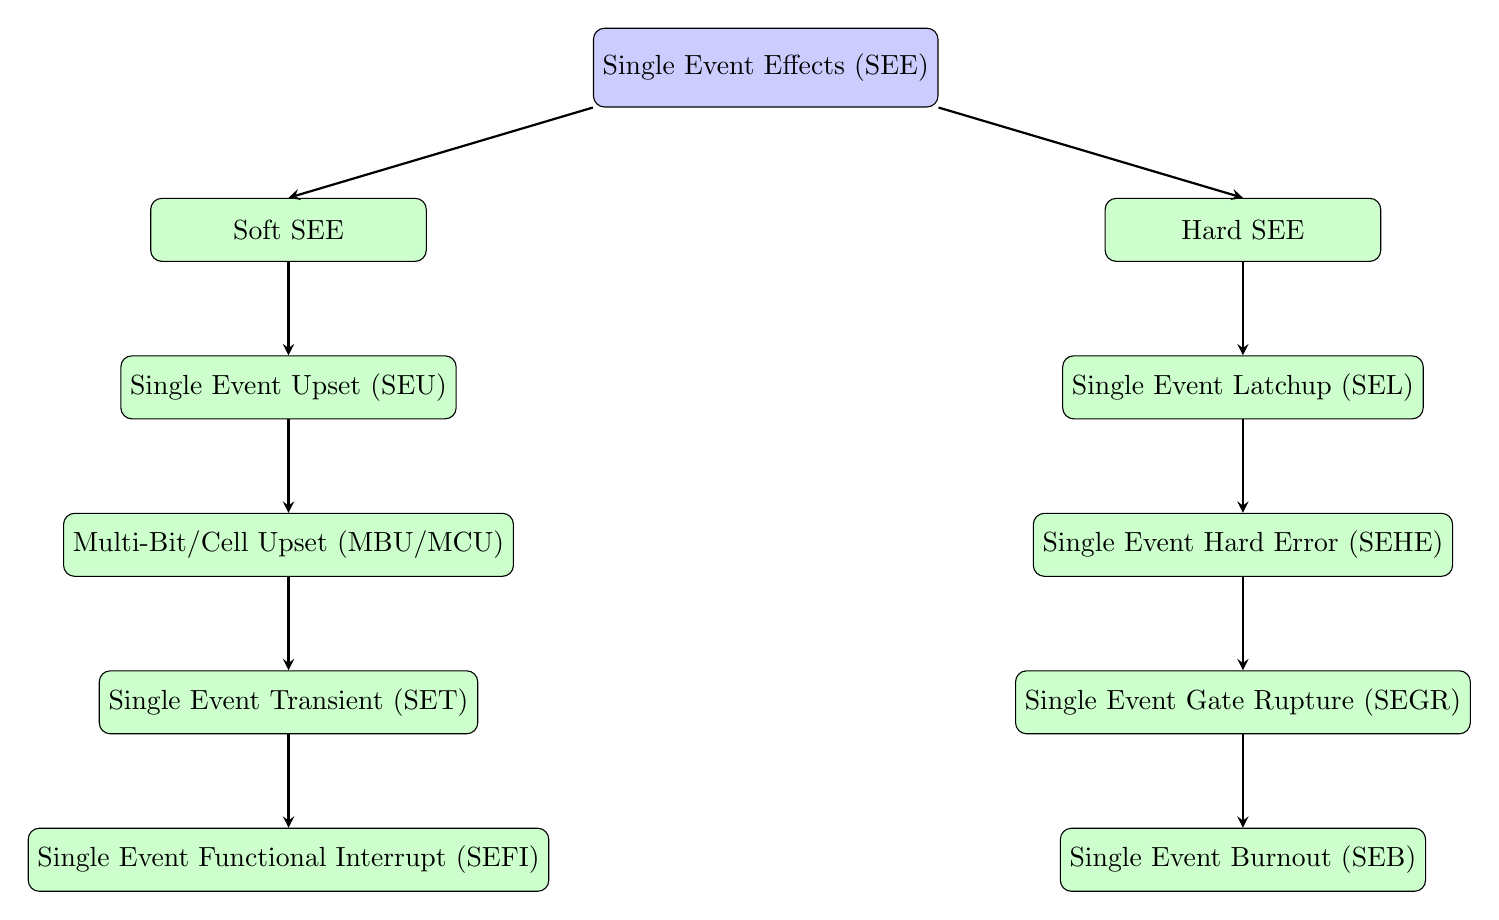
\begin{tikzpicture}[node distance=1.5cm]

% Top-level SEE
\node (see) [block] {Single Event Effects (SEE)};

% Soft SEE
\node (soft) [subblock, below left of=see, xshift=-5cm, yshift=-1cm] {Soft SEE};
\node (seu) [subblock, below of=soft, yshift=-0.5cm] {Single Event Upset (SEU)};
\node (mbu) [subblock, below of=seu, yshift=-0.5cm] {Multi-Bit/Cell Upset (MBU/MCU)};
\node (set) [subblock, below of=mbu, yshift=-0.5cm] {Single Event Transient (SET)};
\node (sefi_soft) [subblock, below of=set, yshift=-0.5cm] {Single Event Functional Interrupt (SEFI)};

% Hard SEE
\node (hard) [subblock, below right of=see, xshift=5cm, yshift=-1cm] {Hard SEE};
\node (sel) [subblock, below of=hard, yshift=-0.5cm] {Single Event Latchup (SEL)};
\node (sehe) [subblock, below of=sel, yshift=-0.5cm] {Single Event Hard Error (SEHE)};
\node (segr) [subblock, below of=sehe, yshift=-0.5cm] {Single Event Gate Rupture (SEGR)};
\node (seb) [subblock, below of=segr, yshift=-0.5cm] {Single Event Burnout (SEB)};

% Arrows from SEE to Soft and Hard
\draw [arrow] (see.south west) -- (soft.north);
\draw [arrow] (see.south east) -- (hard.north);

% Arrows within Soft SEE
\draw [arrow] (soft.south) -- (seu.north);
\draw [arrow] (seu.south) -- (mbu.north);
\draw [arrow] (mbu.south) -- (set.north);
\draw [arrow] (set.south) -- (sefi_soft.north);

% Arrows within Hard SEE
\draw [arrow] (hard.south) -- (sel.north);
\draw [arrow] (sel.south) -- (sehe.north);
\draw [arrow] (sehe.south) -- (segr.north);
\draw [arrow] (segr.south) -- (seb.north);

\end{tikzpicture}
\end{adjustbox}
\caption{Classification of \gls{see} subtypes.}
\label{fig:see_hard_soft}
\end{figure}


This research focuses exclusively on soft errors, while hard errors are beyond the scope of this study and will not be discussed further.

\subsection{Single Event Upsets (SEUs) and Failure Modes}

Most modern high-density \glspl{fpga} rely on \gls{sram} cells to store their configuration bitstream. 

This \gls{cram} defines the functionality of logic blocks (\glspl{lut} and \glspl{ff}) and all internal interconnections. 

Unfortunately, this reliance on volatile SRAM renders \glspl{fpga} highly susceptible to soft errors induced by high-energy ionizing radiation, a phenomenon particularly severe in environments such as space.

As technology feature size decreases, \glspl{seu} and \glspl{set} become the dominant radiation-induced effects in modern microelectronic circuits. In addition, \glspl{mbu}—events in which multiple configuration or memory bits are simultaneously affected—are increasingly significant due to the higher integration density and reduced node capacitance of advanced semiconductor technologies \cite{Zhao2015_SEU_AdvancedIC}.

\subsubsection{Single Event Upsets (SEUs)}

The principal threat to \glspl{fpga} reliability is the \textit{Single Event Upset (SEU)}, a non-destructive event where a single particle strike flips the state of a memory bit \cite{Wilson2025}. In \gls{sram}-based \glspl{fpga}, \glspl{seu} are a major concern because altered configuration bits can permanently change the implemented logic and routing, leading to persistent malfunctions, as illustrated in Figures~\ref{fpga-seu-and} and~\ref{fpga-3upsets-cram}.

\subsubsection{\glsentrytext{see} Induced System Failure Types}

When a \gls{seu} hits an essential or critical bit of the \gls{fpga}'s \gls{cram}, it could change the implemented circuit, altering the expected behavior of the affected area.

The change could affect any of the configurable elements of \gls{fpga}, such as the state of the interconnection switches, the clock configuration, the contents of \gls{bram}, the entries in \gls{lut}, or the specific state of the hardware configuration.

Figure~\ref{fpga-seu-and}(a) illustrates a scenario in which a 2-input \gls{lut} is configured by the \gls{cram} bits to describe an $AND$ gate and the \gls{lut} inputs are connected to the inputs $A$ and $B$ by an interconnection switch.

From Table~\ref{tab:logic_gates}, it is evident that the implemented circuit acts as an $AND$ gate, exhibiting the exact behavior described for the values of its inputs.

Then in Figure~\ref{fpga-seu-and}(b), a \gls{seu} is represented, changing the first value of the 2-input \gls{lut} from $0$ to $1$. Now, the behavior of the circuit changes, as demonstrated in Table~\ref{tab:logic_gates}, from an $AND$ gate to a $XNOR$ gate.

Figure~\ref{fpga-seu-and}(c) illustrates another possible scenario, where an interconnection switch is hit by a \gls{seu}, disconnecting the $A$ input from the \gls{lut}. As the input is left floating, the output result is unpredictable. The unconnected input might drift between high or low logic values, depending on nearby static fields. In the worst case, it drifts to an intermediate voltage and only partially switches the output, leading to excess heating of the gate. Or, the output could oscillate between high and low logic values.

\begin{figure}[ht]
\centering
\includegraphics[width=0.75\textwidth]{Cap3/1-s2.0-S014193312300087X-gr1_lrg.jpg}
\caption{Illustartion o a \gls{seu} effect in a \gls{lut} \gls{fpga} . Adapted from \textcite{Mousavi2023_MTTR_FPGA_Scrubbing}.}\label{fpga-seu-and}
\end{figure}

\begin{table}[ht!]
\centering
\caption{Truth Tables for AND and XNOR Logic Gates.}
\label{tab:logic_gates}
\[
\begin{array}{c c | c @{\hskip 1cm} c c | c}
\multicolumn{3}{c}{\textbf{AND Gate}} & \multicolumn{3}{c}{\textbf{XNOR Gate}} \\
\text{In1} & \text{In2} & \text{Out} & \text{In1} & \text{In2} & \text{Out} \\
\midrule
0 & 0 & 0 & 0 & 0 & 1 \\
0 & 1 & 0 & 0 & 1 & 0 \\
1 & 0 & 0 & 1 & 0 & 0 \\
1 & 1 & 1 & 1 & 1 & 1 \\
\end{array}
\]
\end{table}

\begin{figure}[ht]
\centering
\includegraphics[width=0.75\textwidth]{Cap3/seu-sb-mb.png}
\caption{\gls{sbu} and \gls{mbu} representations in a \gls{fpga} \gls{cram}. Reproduced from \textcite{Aguiar2025_SEE_Space_to_Accelerator}.}\label{fpga-seu-and-sbu-mbu}
\end{figure}

\begin{figure}[ht]
\centering
\includegraphics[width=0.75\textwidth]{Cap3/fncom-17-1268374-g0001.jpg}
\caption{Representation of different types of upsets in a \gls{fpga} \gls{cram}. Reproduced from \textcite{Xie2023_HybridGrainedScrubbing}.}\label{fpga-3upsets-cram}
\end{figure}

\section{Reliability Challenges in SRAM-based FPGAs}

SRAM-based \glspl{fpga} are widely adopted for their flexibility, performance, and reconfigurability. However, their configuration memory (\gls{cram}) and user logic are highly susceptible to soft errors induced by radiation, electromagnetic interference, or aging effects. These transient faults can alter logic functionality or corrupt stored data, potentially leading to malfunction or complete system failure. Understanding the nature, frequency, and impact of these faults is critical to developing effective mitigation strategies.

The concept of soft error criticality describes the potential of \gls{fpga} bits to cause design failures. Upsets in unused regions generally pose a lower risk, as these bits are not expected to affect functionality; however, soft errors could still impact the design if unused elements become inadvertently enabled. Bits configured for the implemented design, whether set to zero or one, are referred to as essential bits. Single-bit upsets in essential bits may be masked by the design, but multiple upsets can accumulate and overcome this inherent protection, potentially leading to errors. Critical bits are those whose flipping can directly cause a system failure, meaning that a single-bit upset in such a bit may compromise the design \cite{Adria2023}. Figure~\ref{fpga-bits-definition} illustrates the classification of the various types of \gls{fpga} bits.

\begin{figure}[ht]
\centering
\includegraphics[width=0.75\textwidth]{Cap3/fpga-bits-definition.png}
\caption{Representation of different types of bits in the \gls{fpga} \gls{cram} due to its criticality. Reproduced from \textcite{Adria2023}.}\label{fpga-bits-definition}
\end{figure}

%%%%%%%%%%%%%%%%%%%%%%%%%%%%%%%%%%%%%%%%%%%%%%%%%%%%%%%%%%%%%%%%%%%%%%%%%%%

\section{N-Modular Redundancy (NMR)}
\gls{nmr} is a fault-masking technique in which multiple identical modules operate in parallel and a majority voter determines the correct output. Although \gls{tmr} (Triple Modular Redundancy) is the most common case, extending to higher-order NMR provides increased fault tolerance at the expense of resource overhead. This section explains the mathematical basis of NMR, voter design considerations, fault coverage properties, and limitations with respect to permanent resource degradation.

\subsection{Voters}

In \gls{nmr} architectures, the \emph{voter} is a fundamental component responsible for determining the final output of the system based on the responses of redundant modules. Mediates the outputs of multiple redundant units to produce a single reliable system response, serving as the coupling element between redundancy and output. Voters are indispensable in both static and hybrid redundancy schemes.

The main functions of voters include the following:

\begin{itemize}
    \item \textbf{Generating Consensus:} Voters receive outputs from the redundant modules and compare them to determine a consensus result, typically based on a majority of matching outputs \cite{Yaman2022,7948063,Dorflinger2022}.
    \item \textbf{Masking Errors:} In a \gls{tmr} configuration, the voter masks single faults by selecting the majority output from the correctly functioning modules, maintaining system reliability \cite{7948063,Yaman2022,Neves2009,OliveiraKastensmidt2023,Wilson2021_TMRVexRiscv}.
    \item \textbf{Propagating the Correct Signal:} Once a consensus is established, the voter propagates the signal identified as correct to the subsequent system stage \cite{Romero2015}.
    \item \textbf{Defining Output Conditions:} In an $N$-modular system, a consensus is achieved when at least $N/2 + 1$ modules produce matching outputs. If this condition is not met, the system is considered to have no valid consensus \cite{Neves2009}.
\end{itemize}

\subsection{Voter Architectures and Vulnerabilities}
\label{sec:voter_types}

Voters play a central role in ensuring reliable outputs in \gls{nmr} systems by mediating between redundant modules. Different voter architectures have been proposed to address specific design constraints and reliability requirements:

\begin{itemize}
    \item \textbf{Majority or Bit-by-Bit Voters:} The majority voter implements the majority function using standard logic gates, such as AND-OR or NAND structures, to determine the final system output based on the majority of identical input values. In wide data buses, this logic can be applied on a bit-by-bit basis, comparing each bit of the outputs individually. Bit-by-bit majority voters are simple and efficient for small or low-throughput systems but may become less effective in high-bandwidth or complex designs due to the lack of word-level integrity verification.

The Boolean equation for a three-input majority voter can be expressed as:
    \begin{equation}
        Q = AB + AC + BC
        \label{eq:maj_voter}
    \end{equation}
    where $A$, $B$, and $C$ represent the outputs of the redundant modules, and $Q$ is the resulting voted output.
    
    For a general case with $N$ redundant modules, the majority function can be defined as:
    \begin{equation}
        Q =
            \begin{cases}
                1, & \text{if } \displaystyle \sum_{i=1}^{N} x_i \geq \left\lceil \frac{N}{2} \right\rceil, \\[6pt]
                0, & \text{otherwise.}
            \end{cases}
    \label{eq:n_input_majority}
    \end{equation}
    where $x_i$ represents the binary output of the $i$-th module, and $Q$ is asserted when the majority of inputs are logical ‘1’.
    
    \item \textbf{Word Voter:} Proposed by \textcite{Mitra2000}, it is designed to overcome the limitations of bit-by-bit voters in wide memory buses, the word voter incorporates additional circuitry to generate an error signal when data integrity is compromised, even by a single-bit fault. This mechanism enhances reliability by revealing inconsistencies that conventional voters may otherwise mask.

   he operation of a three-input word voter can be expressed as:
\begin{equation}
\begin{aligned}
W_{\text{out}} &=
\begin{cases}
W_1, & \text{if } (W_1 = W_3), \\[4pt]
W_2, & \text{if } (W_1 \neq W_3), \\[4pt]
\text{undefined}, & \text{otherwise,}
\end{cases} \\[6pt]
E_{\text{flag}} &= 
\begin{cases}
1, & \text{if } (W_1 \neq W_2) \lor (W_1 \neq W_3) \lor (W_2 \neq W_3), \\[4pt]
0, & \text{otherwise.}
\end{cases}
\end{aligned}
\label{eq:word_voter_mitra}
\end{equation}

where $W_1$, $W_2$, and $W_3$ are the $m$-bit words from the three redundant modules, $W_{\text{out}}$ is the voted output word, and $E_{\text{flag}}$ indicates a mismatch among all module outputs.

This approach enhances data integrity by enabling fault detection at the word level, allowing the system to identify inconsistencies that bit-by-bit voting may overlook.
    
    \item \textbf{Self-Adapted Voter (SAv):} Proposed by \textcite{Tarrillo2014, Tarrillo2014_Power_nMR}, it is designed to tolerates multiple accumulated faults. The SAv determines the output by considering only the responses of healthy modules as part of the majority voting population. It computes the fault-free output (FFO) bit-by-bit based on the summation of outputs from fault-free modules and their total count.
\end{itemize}

\begin{longtable}{|p{3.5cm}|p{2.5cm}|p{2.5cm}|p{2.5cm}|p{2.5cm}|}
\caption{Comparison between fault-free and faulty outputs for each module with voter decisions. Adapted from \textcite{Yaman2022}.}
\label{tab:voter_comparison} \\

\toprule
\textbf{Module} & 
\textbf{0-Module Faulty} & 
\textbf{1-Module Faulty} & 
\textbf{2-Module Faulty} & 
\textbf{3-Module Faulty} \\  
\midrule
\endfirsthead

\multicolumn{5}{c}{\tablename\ \thetable{} -- \textit{continued from previous page}} \\ 
\toprule
\textbf{Module} & 
\textbf{0-Module Faulty} & 
\textbf{1-Module Faulty} & 
\textbf{2-Module Faulty} & 
\textbf{3-Module Faulty} \\ 
\midrule
\endhead

\midrule
\multicolumn{5}{r}{\textit{Continued on next page}} \\ 
\endfoot

\bottomrule
\endlastfoot

A & 000 & 001 & 001 & 100 \\
B & 000 & 000 & 010 & 001 \\
C & 000 & 000 & 000 & 010 \\
\textbf{Majority Voter} & 000 & 000 & 000 & 000 \\
\textbf{Word Voter} & 000 & 000 & \textit{No majority} & \textit{No majority} \\

\end{longtable}

In Table~\ref{tab:voter_comparison}, the design and functionality of word and a bit-by-bit voter architectures are compared. The \emph{word voter} is specifically developed to address limitations associated with bit-by-bit voters in wide memory buses. Unlike conventional designs, word voters incorporate additional circuitry to generate an error signal when data integrity is compromised, even by a single-bit fault. This enhancement significantly improves reliability by detecting inconsistencies that traditional bit-by-bit voters may fail to expose, thereby increasing the overall robustness of the redundant system.

\subsubsection{Voter Vulnerabilities and Mitigation}
Voters are inherently critical components, as they introduce a \textit{single point of failure (SPOF)} within redundant systems \cite{Tarrillo2014,leipnitz2015,Yaman2022,Oliveira2017}. A fault in the voter can compromise the entire redundancy scheme by propagating erroneous results to the system output. For instance, in a \gls{tmr} configuration, an upset in the voter logic renders the redundancy ineffective \cite{Kastensmidt2006}, allowing faulty data to dominate the output. Because the voter's reliability ($R_{\text{voter}}$) directly determines the overall system reliability, enhancing voter robustness through techniques such as redundancy within the voter, temporal voting, or error detection mechanisms is essential for maintaining system dependability.

\section{Dynamic Partial Reconfiguration (DPR)}
\gls{dpr} enables the selective reprogramming of specific \gls{fpga} regions during runtime without disrupting the operation of unaffected modules \cite{Bonna2021}. By targeting only the faulty portions of the design, DPR reduces downtime and resource waste compared to full device reprogramming. This section describes the internal mechanisms of DPR, design partitioning strategies, and how it complements redundancy to achieve self-repairing \gls{fpga} systems.

\begin{figure}
    \centering
    \includegraphics[width=1\linewidth]{Cap3/dpr-xilinx.png}
    \caption{Basic Principle of \gls{dpr}.Reproduced from \cite{Xilinx_UG702_PR}.}
    \label{fig:dpr-xilinx}
\end{figure}

\gls{dpr} is a powerful feature widely adopted in modern embedded systems and hardware prototyping, particularly in designs based on \glspl{sram}-based \glspl{fpga}. It enables the modification of hardware functionality at runtime without interrupting the operation of the remaining system components \cite{Ghaffari2014_FastSRAM_FI,ZanoneSaotome2023,Wilson2020_VideoPipelines}.

\subsection{Definition and Mechanism}
\gls{dpr} allows specific regions of the \gls{fpga} fabric to be reconfigured while other regions continue operating normally \cite{Bonna2021,ZanoneSaotome2023,Barbosa2021}. This capability makes it a cornerstone of runtime-reconfigurable embedded systems, enabling computing devices to modify their hardware architecture dynamically according to application demands.

The main characteristics of \gls{dpr} include:
\begin{itemize}
    \item \textbf{Selective Modification:} Enables the reconfiguration of a defined region within the \gls{fpga} without interrupting the operation of the rest of the device \cite{Barbosa2021,Wilson2020_VideoPipelines}.
    \item \textbf{Partitioning:} The programmable area can be divided into one or more partitions, where each partition can be reconfigured independently \cite{Bonna2021}. These reconfigurable regions are typically defined using Vivado’s \texttt{pblock} feature \cite{Wilson2020_VideoPipelines}.
    \item \textbf{Static and Dynamic Logic:} \gls{dpr} separates the design into static (fixed) logic and dynamic (reconfigurable) logic. The static logic remains constant, while the dynamic logic—implemented in \glspl{dpr} can be replaced or updated at runtime \cite{Wilson2020_VideoPipelines}.
    \item \textbf{Partial Bitstreams:} Reconfiguration is performed through the loading of partial bitstreams, which contain only the configuration data for the reconfigurable partition, unlike full bitstreams that include both static and dynamic regions \cite{Yang2022_FaultInjectionUltrascale}.
\end{itemize}

Figure~\ref{fig:dpr-xilinx} illustrates the concept described above, where multiple partial bitstreams can coexist in external memory and dynamically loaded, one at a time, into the reconfigurable region of the \gls{dpr} setup.

\subsection{Implementation in FPGA Platforms}
Implementing \gls{dpr} requires dedicated configuration flows and access to the device’s configuration memory through specialized interfaces. The most common configuration interfaces include:

\begin{itemize}
    \item \textbf{Internal Configuration Access Port (ICAP):}  
    An internal hardware interface accessible through HDL primitives. The ICAP allows rapid reconfiguration directly from within the programmable logic and is often employed in fault injection or fast module updates.

    \item \textbf{Processor Configuration Access Port (PCAP):}  
    Available on Xilinx Zynq and UltraScale+ \glspl{fpga}, the PCAP is managed by software running on the embedded ARM processor. It facilitates bitstream transfer between the Processing System (PS) and the Programmable Logic (PL) via DMA, enabling efficient runtime reconfiguration.

    \item \textbf{JTAG and SelectMAP:}  
    External configuration interfaces commonly used for debugging, testing, or initial configuration. While JTAG offers flexibility for development and validation, SelectMAP provides higher bandwidth for bitstream loading during operation.
\end{itemize}

Thus, \gls{dpr} provides a foundation for adaptive and fault-tolerant \gls{fpga} systems, enabling the replacement, recovery, or upgrade of hardware modules on demand without system downtime.

\section{Memory Scrubbing Techniques}
Configuration memory scrubbing is a proactive approach that periodically reads and corrects the \gls{fpga} configuration to prevent error accumulation. This section discusses different scrubbing approaches, including blind scrubbing, readback-and-verify, and adaptive scrubbing. It also analyzes trade-offs between error coverage, bandwidth consumption, and system availability.

\subsection{Scrubbing in SRAM-Based FPGAs}

According to \textcite{Wubs2023}, the primary method for correcting bit-flips in the configuration memory of \glspl{fpga} based on \gls{sram} technology is \emph{scrubbing}. This process consists of rewriting corrupted configuration frames using a radiation-protected reference. Faults are identified either through continuous comparison between the current configuration memory and the reference, or by employing \glspl{ecc} mechanisms.

Two main approaches to scrubbing exist: internal and external. Internal scrubbers leverage the \gls{fpga}’s own resources and require no additional hardware but generally provide limited fault detection and correction capabilities. In contrast, external scrubbers offer higher performance and reliability, though they require dedicated external hardware to manage the process.

Scrubbing can be performed on the entire configuration memory (\emph{full scrubbing}) or on selected regions (\emph{partial scrubbing}). The latter is only feasible if the targeted area is physically isolated from the rest of the circuit to avoid interference. It is important to note that scrubbing merely prevents the accumulation of soft errors in configuration memory. Bit-flips that occur between scrubbing cycles can still cause functional errors or incorrect output states, since there is an inevitable latency between fault occurrence and correction. Moreover, scrubbing does not address faults in user registers or embedded memories, which remain susceptible to radiation-induced effects~\cite{Wubs2023}.

As highlighted by \textcite{Adria2023}, \glspl{seu} in \glspl{fpga} may lead to persistent functional errors by altering the architectural configuration of the implemented design. To mitigate such effects and prevent fault accumulation, \gls{cram} scrubbing is a well-established corrective strategy. However, scrubbing does not prevent the occurrence of bit-flips, nor can it fully mitigate the consequences of upsets affecting critical bits. Therefore, additional design-level mitigation mechanisms are typically employed to reduce single points of failure and enhance the system’s fault-masking capability.

Several scrubbing architectures have been proposed in the literature, differing mainly in their error detection methods, resource utilization, power consumption, and correction latency~\cite{heiner2008,Brosser2014,tonfat2015,7776929}. Scrubbing strategies are usually classified into two categories:
\begin{itemize}
    \item \textbf{Internal scrubbing:} The scrubber engine is implemented within the same \gls{fpga} that it monitors. This approach requires no additional hardware and provides high-speed detection and correction capabilities. An example is the \gls{semip}~\cite{amd2023sem}, which is integrated into most modern Xilinx devices. However, internal scrubbers remain vulnerable to \glspl{seu} that may affect their own logic or communication interfaces. Such upsets may cause the scrubber to become unresponsive, compromising its correction capability, especially in cases involving multiple simultaneous upsets~\cite{berg2008}.
    \item \textbf{External scrubbing:} The scrubber controller is implemented on an external device. This architecture provides greater robustness and can manage multiple upsets more reliably, as it is isolated from the internal \gls{fpga} logic.
\end{itemize}

\begin{figure}
    \centering
    \includegraphics[width=1\linewidth]{Cap3/scrubbing1.30.png}
    \caption{Different memory scrubbing techniques, (a) Internal (b) External.}
    \label{fig:scrubbing-int-ext}
\end{figure}

\begin{figure}
    \centering
    \includegraphics[width=0.5\linewidth]{Cap3/scrubbing2-30.png}
    \caption{Scrubbing method available in \gls{soc} devices.}
    \label{fig:scrubbing-soc}
\end{figure}

However, \gls{cram} scrubbing, whether internal or external, does not protect volatile memory elements such as \glspl{bram}, distributed memories (\glspl{lutram}) and \glspl{ff}. Upsets in these dynamic elements must be addressed through complementary techniques such as redundancy, \gls{ecc}, or periodic resets to restore the initial state of the system. In more severe cases, such as \glspl{sefi} that affects the control logic or configuration interfaces \gls{fpga}, a power cycle may be required to restore normal operation.

\bigskip
\noindent
Although scrubbing plays a crucial role in preventing the accumulation of faults in configuration memory, it does not offer insight into how these issues affect system functionality or reliability at the architectural level. To evaluate and validate the effectiveness of mitigation techniques, researchers often employ \emph{\gls{fi}} campaigns. The next section explores \gls{fi} as an essential experimental approach for characterizing fault tolerance and assessing the dependability of \gls{fpga}-based systems.

\section{Fault Injection Principles}
Fault injection is an essential method to evaluate the robustness of fault-tolerant \gls{fpga} designs. By deliberately introducing controlled errors into the system, researchers can analyze failure modes, verify mitigation strategies, and quantify reliability metrics. This section explains fault injection models (bit-flip, stuck-at), implementation techniques (simulation-based, emulation-based, on-chip), and evaluation criteria.

\subsection{Fault Injection in FPGA-Based Systems}

According to \textcite{Adria2023}, \gls{fi} is an experimental technique used to deliberately introduce faults into a system to reproduce radiation-induced effects and evaluate the dependability of its design. It serves to identify vulnerable regions that require hardening and to validate the effectiveness of implemented fault-mitigation strategies. In radiation-tolerant applications, \gls{fi} is an essential step in characterizing failure mechanisms, validating recovery techniques, and assessing system-level robustness~\cite{Adria2023,leipnitz2015}.

Fault injection can be applied at various abstraction levels, including transistor, gate, register-transfer (RTL), or system level~\cite{anghel2007}. For example, in a soft processor implemented in a \gls{sram}-based \gls{fpga}, bit flips injected into \gls{cram} affect the processor’s \gls{rtl} architecture, while faults injected into \glspl{bram} influence the execution of applications at the user-level~\cite{Adria2023}.

Different techniques can be used to perform fault injection, depending on the level of realism, controllability, and available hardware resources. The three main approaches are as follows:

\begin{itemize}
    \item \textbf{Physical fault injection:} faults are induced through direct physical means, such as heavy-ion or proton irradiation, laser strikes, or voltage and electromagnetic perturbations. This method offers the highest realism since it reproduces actual radiation effects, but requires specialized facilities and equipment, often resulting in limited controllability and higher cost~\cite{Adria2023,Fibichi2019}.
    
    \item \textbf{Simulation-based fault injection:} faults are introduced within simulation environments or hardware description language (HDL) models. This approach provides full observability and high controllability, enabling exhaustive testing at the cost of reduced execution speed and limited hardware fidelity~\cite{Adria2023,Fibichi2019}.
    
    \item \textbf{Emulation-based fault injection:} faults are injected directly into a running hardware prototype, typically implemented on an \gls{fpga}. This technique offers a balance between accuracy and performance, allowing real-time experimentation under conditions close to the actual operation. It enables efficient evaluation of mitigation schemes such as redundancy, scrubbing, and dynamic partial reconfiguration (\gls{dpr})~\cite{Adria2023,Fibichi2019}.
\end{itemize}

Fault injection can also be classified based on the injection controller architecture. Hardware-based injectors use an external module that introduces faults without disturbing the system’s normal operation, while software-based injectors operate within the target device and may temporarily pause its execution to perform the injection~\cite{velazco2000}. The latter are more intrusive but easier to implement, whereas hardware injectors are non-intrusive and provide better temporal precision.

In addition, fault injection strategies can be either \emph{deterministic} or \emph{random}. Deterministic injections target predefined configuration bits or memory elements, enabling controlled evaluation of specific fault locations. Random injections, in contrast, select bits probabilistically to emulate stochastic radiation-induced events. Exhaustive single-bit injections are often used to identify critical configuration bits in the design, while accumulative random injections allow faults to build up over time, offering insight into the system’s behavior under multiple concurrent upsets~\cite{benevenuti2019}.

The temporal aspect of fault injection is also crucial. The timing of an injected fault within a clock cycle or during software execution can greatly influence whether it propagates, becomes masked, or leads to a system failure~\cite{quinn2013}. Therefore, a realistic fault-injection campaign must statistically cover both spatial and temporal domains to faithfully reproduce radiation-induced behavior.

Among these methodologies, emulation-based \gls{fi} has become particularly valuable for evaluating \gls{fpga}-based systems. It allows for real-time fault-effect observation, short testing cycles, and validation of fault-tolerance strategies such as modular redundancy, scrubbing, and \gls{dpr}. In this work, \gls{fi} is employed as a key validation mechanism to characterize the fault tolerance of \gls{fpga}-based designs and to assess the reliability enhancements achieved through redundancy and \gls{dpr} techniques.

\section{Physical Mitigation Techniques}

Mitigation through physical protection can take several forms, including traditional physical barriers, technological fabrication improvements, and layout- or placement-level design strategies. These approaches aim to reduce the impact of radiation by either preventing particle interaction with sensitive regions or by hardening the device structure to withstand such interactions.

\subsection{Physical Barriers and Material-Based Hardening}
Historically, physical protection through shielding was one of the first techniques used to mitigate \glspl{seu} in spacecraft, effectively reducing the incident particle flux. However, the efficiency of shielding depends strongly on the type of radiation involved:
\begin{itemize}
    \item Shielding is effective against alpha and beta particles but has limited effect against gamma rays, neutrons, or heavy ions \cite{Barbosa2021}.
    \item Even with duplication or triplication of shielding layers, the reduction in proton-induced effects is often marginal \cite{Barbosa2021}..
    \item Additional insulating and polymer-based materials have been explored to mitigate soft errors, though their effectiveness remains application-dependent \cite{Rogenmoser2023_HMR,Barbosa2021}.
\end{itemize}

At the device manufacturing level, protection is achieved through \gls{rhbp}. These techniques mitigate \gls{tid} and \gls{sel} effects by modifying fabrication processes, such as using \gls{soi}, \gls{bicmos}, or other wide-bandgap technologies. \gls{rhbp} acts directly on oxide and interface charge-retention characteristics, while structural modifications like isolation wells or current-limiting transistors can prevent destructive latch-up events \cite{Barbosa2021}..

\subsection{Hardening by Physical Design and Layout}
Another level of mitigation, known as \gls{rhbd}, focuses on the physical layout of the circuit to improve resilience against radiation effects \cite{Rogenmoser2023_HMR}:
\begin{itemize}
    \item \textbf{Layout Modification:} Increasing the spacing between sensitive nodes reduces charge sharing from particle strikes, while enlarging transistors in critical paths increases their critical charge ($Q_{\text{crit}}$), enhancing radiation tolerance \cite{Battezzati2010}.
    \item \textbf{SEL Detection and Limitation:} External circuitry on the power rails can detect abnormal current spikes caused by latch-up and act as resettable fuses or current limiters \cite{Battezzati2010}.
    \item \textbf{SET Mitigation:} Proper contact placement and signal routing can help cancel transient pulses generated by radiation events \cite{Sharma2020_IPFA_MBU}.
\end{itemize}

\subsection{SEU-Aware Placement}
A modern design-flow-level mitigation approach, proposed by \textcite{Wilson2025}, is the \gls{seu}-aware placement, which applies physical placement constraints during the implementation phase:
\begin{itemize}
    \item This method improves fault tolerance without modifying the \gls{hdl}'s design source code.
    \item Using \gls{xdc} or \gls{tcl} scripts, designers can control the placement of logic elements, registers, and routing paths to minimize sensitivity to \glspl{seu}.
    \item It also enables \textit{domain striping}---the physical separation of redundant modules---and prevents optimization tools from merging triplicated elements such as global clock buffers, thereby maintaining redundancy integrity.
\end{itemize}

Physical protection and mitigation strategies, such as shielding and material hardening, are commonly employed to reduce radiation-induced effects at the device level by attenuating or blocking incident particles, thereby minimizing the probability of single-event phenomena. Although these techniques play an important role in enhancing device resilience, this research does not focus on such approaches. Mitigations based on external barriers or material hardening are beyond the scope of this work, which instead emphasizes architectural and logic-level strategies, particularly those involving \gls{nmr} and \gls{dpr}.